\section{Execution Layers}
\label{subsec:detailed_execution_layers}
The execution layers is NOX ECS's way of supporting the requirement for multi-threading,
without requiring large investments for the user\reqref{req:multi_threading}.

\subsection{Explanation}
The execution layers is a structure detailing which components types can be run concurrently.
The structure consist of one or more layers, where each layer has a set of component types.
Each set of component types can be run concurrently.
When all the component types in one layer has been executed, the next layer can be started.
The sets are created through an algorithm that finds out which component types can be run concurrently,
based on information given by the programmer.

\begin{figure}[tbp]
    \begin{center}
    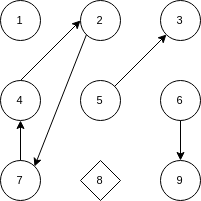
\includegraphics[scale=0.45]{images/layered_execution_model_1.png}
    \caption[Execution layers, not layered]{Component Collection Lifecycle Partitioning}
    \label{fig:execution_layers_model_1}
    \end{center}
\end{figure}

\begin{figure}[tbp]
    \begin{center}
    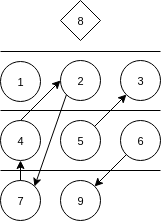
\includegraphics[scale=0.45]{images/layered_execution_model_2.png}
    \caption{Component Collection Lifecycle Partitioning}
    \label{fig:execution_layers_model_2}
    \end{center}
\end{figure}

\subsubsection{Component Access}
\label{subsec:detailed_component_access_levels}
Describing the actions executed on different components is done with the data access enum, which has 4 values.

\begin{itemize}
    \item unknown\\
    All component types are marked as unknown by default, as per the opt-in policy\secref{subsec:high_level_intention}.
    This data access states that there is nothing known about the components access patterns.
    Every component type marked with unknown is therefore put into its own separate layer, as they are interpreted to be reading from all other components.
    Unknown component types are treated like this because expecting the worst case scenario is the only way to ensure the program is run correctly.

    \item read and write\\
    Read and write data access is planned to be implemented in the future, and currently follows the same logic as unknown.
    This is because the algorithm could be extended to take writes into account, instead of only dealing with reads.
    If this was implemented, each component type would need an additional list for which components are written to,
    as the writes would have to be treated differently from reads.

    \item read only\\
    A component that only reads from others can be marked read only. This means that it can be put on any layer, as long
    as it does not read from any other components on that layer.

    \item independent\\
    A component marked as independent can be run in any layer, as long as no other components on that layer reads from it.
\end{itemize}

\subsubsection{Read list}
\label{subsec:detailed_read_list}
Each component with read access has its own read list that is defined by the programmer.
The list contains all other components types that the component type in question reads from.
The algorithm uses the read list to figure out how the layers should be structured.

\subsubsection{Important qualities of the structure}
There are a few qualities that the structure both needs, and should have in order to perform better.

\paragraph{No same layer read connections}
It is important that no component types has connections to components in the same layer.
This would cause issues if a component changes one of its own member variables, and another component reads from it.
Allowing these same layer reads would start creating race conditions.

\paragraph{Per layer component count to thread count ratio}
The number of component types in each layer should optimally be divisible by the amount of threads available.
A mismatch between the number of component types and threads available would lead to some threads having to wait while the other threads finish their work.
For example if there are 5 component types in a lair, with each type requiring the same work load to finish, and there are 3 worker threads.
After the initial 3 component types are finished, 1 thread has to wait while the two others finish the remaining component.
It would have been better to reduce the size of the layer to 3, and move the excess components to other layers trying to have a component type count divisible by the thread count.
There will always be some time spent waiting on other threads to finish before moving onto the next layer, but following this rule will reduce this waiting.

\subsubsection{The algorithm}
The algorithm itself that creates and sets up the execution layer structure goes through three stages: The data collection stage, layer creation stage, and parsing stage.

\paragraph{Data collection stage}
This stage consists of setting up all the data needed to run the algorithm.
The algorithm gets the access levels to each component type, and which other components they have read connections to.
If the component type is any other than read only, certain actions will be taken, as mentioned in the component access levels\footnote{See p.\pageref{subsec:detailed_component_access_levels}}.
In the case of having independent data access, the whole read list is simply emptied.
Having either unknown or read and write will result in the component type having its own separate layer.

%\subsubsection{Initialize data}
%\lstinputlisting[language=cpp, caption=initialize data, label=lst:initialize_data]{initialize_data.py}

\paragraph{Layer creation stage}
The algorithm goes through all the component types and creates layers.
This is done in the following steps.

\begin{enumerate}
    \item Picking out the component with the most connections.

    \item Creating a list of remaining components which does not have a colliding connection with the current layer.

    \item Find the component in the list with the fewest additional new connections to the layer, and add it to the layer.

    \item Repeat step 2-3 until there is no components left that can be placed in the list.

    \item Remove excess components in the layer, if it does not match up with the thread count.

    \item Repeat step 1-5 until all components are put into layers.
\end{enumerate}

\paragraph{Data parsing stage}
The data parsing stage turns the layers from type identifiers to indexes used within the entity manager\secref{subsec:detailed_entity_manager}
This format change is favorable as the type identifiers\secref{subsec:detailed_type_identifier} used internally in the algorithm would require a search through the list of component collections\secref{subsec:detailed_component_collection} every frame, rather than just a constant index lookup.

\subsection{Motivation}
The main motivation for this structure was to allow concurrent execution of more components
than just the independent ones.
Having a programmer specifying a read list is an easier way to add concurrency without to much burden on the programmer\reqref{req:multi_threading}.

\subsection{Alternatives}
There are a few alternatives to the existing solution, and all of these are better ways of dealing with the task at hand.
They all either require a lot more work, are hindered due to requirements, or were not prioritized.

\subsubsection{Caching}
One solution could be a caching mechanism, which involves keeping previous frame's data to work on for the next frame\cite[p.930]{game_engine_architecture}.
The main advantages are that synchronization and data races are no longer an issue, as the data being read from will not change during the reads.
In addition to running all components concurrently, it would avoid the possibility of human error from manually defining the read list for each component.
The disadvantage is that the system would require double the amount of memory to save the previous frame.
This also requires all types to be deep copyable.

\subsubsection{Saving execution layer structure}
The execution layers could be saved to file, rather than computing it on every run.
This should both be easy to implement, and completely remove the time to compute the structure when no new changes to the components have been made.

\phantomsection
\subsubsection{Code analysis}
\label{par:detailed_execution_layers_code_analysis}
Code analysis could be added to automatically and reliably find dependencies, removing the need for the programmer to manually specify the read lists and data access for components.
However, implementing this is both very time consuming, and quite difficult as it requires parsing of the C++ language, which is fairly complex.

\subsection{Pros of Execution Layers}
The main pro of the execution layers is the ease adding concurrency functionality for the user,
allowing utilization of multi-core CPU's.

\subsection{Cons}
Adding the support for multi threading components in this manner leads to some disadvantages.

\subsubsection{Increased loading times}
With the execution layers having to be computed at every start up, the load times might increase a bit when adding lots of component types.

\subsubsection{More error prone}
Requiring the programmers to specify data access and the read list manually, can be error prone. This could lead to several bugs caused by human error.
Additionally, the fact that any part of the execution layers structure can vary based on small changes, means that even though an incorrect read list has been specified, a problem may not occur until later changes.
